\documentclass[numbering=fraction]{beamer}
\usetheme[progressbar=frametitle]{metropolis}

\usepackage[bulgarian]{babel}
\usepackage[utf8]{inputenc}
\usepackage[style=alphabetic,backend=biber]{biblatex}
\usepackage{blindtext}
\usepackage{tikz}
\usepackage{progressbar}
\usepackage{amsmath}

\uselanguage{Bulgarian}
\languagepath{Bulgarian}
\providetranslation[to=Bulgarian]{Corollary}{Следствие}

\addbibresource{bibliography.bib}
\graphicspath{{pictures/}}

\title{БЧХ кодове}
\titlegraphic{\vspace{4cm}\flushright
\includegraphics[width=2cm,height=1.25cm]{fmi-logo.png}}
\author[Author]{Кристиян Стоименов}
\institute{Факултет по математика и информатика,\\\textbf{Увод в теорията на кодирането}}
\date{\today{}}

\begin{document}
\definecolor{salmon}{RGB}{255, 128, 128}
\definecolor{darkgrey}{RGB}{50, 50, 50}

\setbeamercolor{frametitle}{fg=darkgrey}
\setbeamercolor{title separator}{fg=salmon}
\setbeamercolor{footline}{fg=darkgrey}
\setbeamercolor{progress bar}{fg=salmon}
\setbeamercolor{alerted text}{fg=salmon}
\setbeamercolor{block title example}{fg=salmon}
\setbeamercolor{section in foot}{fg=white, bg=salmon}

\makeatother
\setbeamertemplate{footline}
{
  \leavevmode%
  \hbox{%
  \begin{beamercolorbox}[wd=.333333\paperwidth,ht=2.25ex,dp=1ex,center]{section in foot}%
    \usebeamerfont{title in foot}К. Стоименов
  \end{beamercolorbox}%
  \begin{beamercolorbox}[wd=.333333\paperwidth,ht=2.25ex,dp=1ex,center]{section in foot}%
      \usebeamerfont{title in foot}\insertshorttitle
  \end{beamercolorbox}%
  \begin{beamercolorbox}[wd=.333333\paperwidth,ht=2.25ex,dp=1ex,right]{section in foot}%
    \insertframenumber{} / \inserttotalframenumber\hspace*{2ex}
  \end{beamercolorbox}}%
  \vskip0pt%
}
\makeatletter
\setbeamertemplate{navigation symbols}{}

\setbeamertemplate{frametitle}
{
\vspace*{16pt}
\Large{\insertframetitle}
% \insertprogressbar
}

\setbeamertemplate{section in toc}{{\color{salmon}\inserttocsectionnumber.}~\inserttocsection}

\setbeamertemplate{caption}{\raggedright\insertcaption\par}


\renewcommand*{\bibfont}{\footnotesize}

\newcommand{\iu}{{i\mkern1mu}}

\newcommand{\rootsofunity}[1] {
\begin{tikzpicture}
  \coordinate (center) at (0, 0);
  \def\radius{2cm}
  \def\n{#1}
  \pgfmathsetmacro\angle{360/\n}
  \pgfmathsetmacro\startangle{90}

  \foreach \i in {0,...,\the\numexpr\n-1\relax} {
    \coordinate (point\i) at ({\startangle+\angle*\i}:\radius);
    \coordinate (label\i) at ({\startangle+\angle*\i}:\radius+0.25cm);
    \node[anchor={\startangle+\angle*\i-90}] at (label\i){$\omega_{\n}^{\the\numexpr\n-\i\relax}$};
    \fill[salmon] (point\i) circle (2pt);
  }

  \draw[salmon, thick] (point0) \foreach \i in {1,...,\the\numexpr\n-1\relax} { -- (point\i) } -- cycle;
  \draw[black, thick] (center) circle (\radius);
  \draw[->] (-2.5,0) -- (2.5,0) node[right] {$\text{x}$};
  \draw[->] (0,-2.5) -- (0,2.5) node[above] {$\text{y}$};
\end{tikzpicture}
}

\newcommand{\floor}[1]{\lfloor #1 \rfloor}


:q
ls


\begin{frame}[plain]{}
\maketitle
\end{frame}

\begin{frame}{}
\section*{Съдържание}
\tableofcontents
\end{frame}

\begin{frame}
\section{История}
\begin{itemize}
    \item БЧХ кодовете са открити от Bose и Ray-Chaudhuri с \autocite{bose1960}, както и независимо от Hocquenghem в \autocite{hocquanghem1959}.
    \item По първоначалните резултати употребата се свежда единствено до бинарни кодове с дължина на кодовите думи $2^m - 1, m \in \mathbb{Z}$.
    \item Впоследствие Gorenstein и Zierler в \autocite{gorenstein1961} разширяват способностите му до $GF(q)$, което в последствие се свързва с развитие на Reed-Solomon кодовете.
\end{itemize}
\end{frame}

\begin{frame}
\begin{minipage}[t]{0.45\linewidth}
\begin{figure}
    \centering
    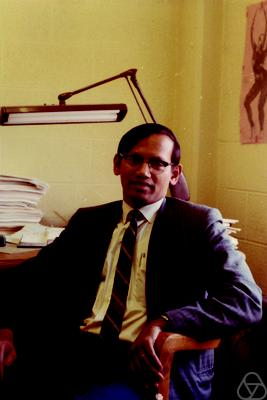
\includegraphics[width=0.5\linewidth]{chaudhui-photo.png}
    \caption{Dijen K. Ray-Chaudhuri - математик, чието име се свързва най-често с решението на т.нар задача на Kirkman за ученичката.}
    \label{fig:chaudhui-photo}
\end{figure}
\end{minipage}%
\hfill
\begin{minipage}[t]{0.45\linewidth}
\begin{figure}
\centering
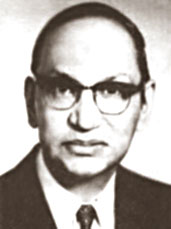
\includegraphics[width=0.5\linewidth]{bose-photo.png}
\caption{Raj Chandra Bose (1901 - 1987) - индийско-американски математик, известен най-вече с ролята си в развитието на БЧХ кодовете и понятието силно свързан граф.}
\label{fig:bose-photo}
\end{figure}
\end{minipage}
\end{frame}

\begin{frame}[plain]
\section{Какво е БЧХ код?}
\end{frame}

\begin{frame}
\begin{definition}
\bigskip
Нека $n$ и $q$ са взаимно прости числа, а $F_{q^m}$ е разширание на $F_q$, което
съдържа всички $n$ корена на полинома $x^n - 1$. Нека също $\alpha$ е
\alt<2->{\alert{примитивен $n$-ти корен на 1}}{примитивен $n$-ти корен на 1} над
полето $F_q$. БЧХ код над $F_q$ с дължина $n$ и \alt<3->{\alert{конструктивно разстояние $\delta$}}{конструктивно разстояние $\delta$}
е \alt<4->{\alert{цикличен код с дължина $n$}}{цикличен код с дължина $n$} и пораждащ полином \[
g(x) = [M_{\alpha^b}(x), M_{\alpha^{b + 1}}(x), \dots, M_{\alpha^{b + \delta
		- 2}}(x)],
\]
където $M_{\alpha^s}$ е \alt<5->{\alert{минималния полином}}{минималния полином} на елемента $\alpha ^ s$ над $F_q$.
\end{definition}
\onslide<6->{\bigskip\emph{Да се опитаме да го дешифрираме.}}
\end{frame}

\begin{frame}{Корени на 1}
\begin{definition}
\smallskip
Ако $n \in \mathbb{N}$, то корените на полинома $x^n - 1$ се наричат \emph{$n$-ти корени на единицата.}
\pause \\
\bigskip
Можем да забележим обаче, че за фиксирано $n$ всички корени са числата
\[
\omega^0, \omega^1, \omega^2, \dots, \omega^{n - 1}
\]при
\[
\omega = \cos{\frac{2\pi}{n}} + \iu\sin{\frac{2\pi}{n}}.
\]
\end{definition}
\end{frame}

\begin{frame}{Корени на 1}
И така получаваме точно елементите на цикличната група $\mathbb{C}_n$. \\

\begin{columns}[T] % align columns
\begin{column}{.48\textwidth}
\begin{figure}
\rootsofunity{5}
\vspace*{-2em}
\caption{Цикличната група $\mathbb{C}_5$}
\end{figure}
\end{column}
\hfill
\begin{column}{.48\textwidth}
\begin{figure}
\rootsofunity{17}
\vspace*{-2em}
\caption{Цикличната група $\mathbb{C}_{17}$}
\end{figure}
\end{column}
\end{columns}

\end{frame}

\begin{frame}{Корени на 1}
За да си обясним какво означава, че корените са \emph{примитивни}, е необходимо
да използваме и следното понятие:
\begin{definition}
\smallskip
Нека $\alpha$ е $n$-ти корен на 1. Казваме, че $\alpha$ принадлежи на
\emph{показател} $d$, ако \[
\begin{cases}
	\alpha^d = 1 \\
	\alpha^m \ne 1 & за 0 < m < d
\end{cases}\]
\bigskip
\underline{т.е} показателят е редът на елемента $\alpha \in \mathbb{C}_n$.
\end{definition}
\end{frame}

\begin{frame}{Корени на 1}
Тогава
\begin{definition}
\smallskip
Ако $\alpha$ принадлежи на показател $n$, ще казваме, че е \emph{примитивен n-ти корен на 1}.
\end{definition}
\smallskip
\underline{т.е} $\alpha$ е примитивен $n$-ти корен на 1 \textit{тстк}
$\mathbb{C}_n = \langle\alpha\rangle$.
\end{frame}

\begin{frame}{Конструктивно разстояние $\delta$}
Това понятие се основава на следното важно твърдение, известно още като БЧХ
граница:
\begin{theorem}
Нека $\alpha$ е примитивен корен на 1 над полето $F_q$. Ако $C$ е цикличен код с
дължина $n$ и пораждащ $g(x)$, за който \[
\exists \delta, b \in \mathbb{Z},
\] такива че \[
g(\alpha^b) = g(\alpha^{b + 1}) = \dots = g(\alpha^{b + \delta - 2}) = 0,
\]
тогава $d(C) >= \delta$.
\end{theorem}
\end{frame}

\begin{frame}{Минимален полином на елемент над поле}
Припомняме, че ако $F_q$ е подполе на $\mathbb{C}$, $F_q < \mathbb{C}$, то число
$\alpha \in \mathbb{C}$ наричаме \emph{алгебричен елемент $F_q$}, ако $\alpha$ е
корен на ненулев $f \in F_q[x]$. \\
\smallskip
Всеки такъв алгебричен елемент си има специален полином, зададен от
следната
\begin{definition}
\smallskip
Ненулевият полином от най-ниска степен, на който $\alpha$ е корен и който е
унитарен\footnotemark, се нарича \emph{минимален полином на $\alpha$ над $F_q$}.
\end{definition}
\footnotetext[1]{Със старши коефициент единица.}
\end{frame}

\begin{frame}{Цикличен код}
Последното понятие, използвано в определението на БЧХ кодове, което не сме
припомнили досега, е \emph{цикличен код}. Макар, че вече го използвахме
неведнъж, го споменаваме накратко, тъй като това е по-общия клас, в който
попада класът на БЧХ кодовете по същия начин както цикличните кодове са по-тесен
клас на линейните блокови. \\
\smallskip
Това означава, че всеки алгоритъм за кодиране и декодиране, свойства и граници на
циклични кодове важи в пълна степен и за БЧХ кодовете, които от своя страна
поради особенностите си предоставят по-ефикасни методи и по-ясни свойства.
\end{frame}

\begin{frame}{Цикличен код}
\begin{definition}
\smallskip
Цикличен код е вид линеен код, за който важи следното свойство. Ако $C$ е
цикличен код, то \[
	\forall c = (a_0, a_1, \dots, a_{n - 1}) \in C
	\implies c' = (a_{n - 1}, a_0, \dots, a_{n - 2}) \in C.
\]
\end{definition}
\smallskip
Някои от по-интересните свойства, които БЧХ кодовете ``наследяват'', поради своята
цикличност включват
\begin{itemize}
	\item съществуване на пораждащ полином,
	\item способност за систематично и несистематично кодиране единствено чрез
	действия с полиноми,
	\item възможност за декодиране чрез декодера на Мегит.
\end{itemize}
\end{frame}

\section{Свойства на БЧХ кодовете}

\begin{frame}{Общо за БЧХ кодовете}
\begin{itemize}
	\item Основната идея на този вид кодове е, че те са циклични кодове, които
	се определят от корените на своя пораждащ полином.
	\item Тяхната главна цел е чрез пораждащия полином $g(x)$ и началната
	стойност $b$, поставена за степен на $\alpha$, да се зададе такова
	конструктивно разстояние $\delta$, че да се състави код със способност за
	поправяне на повече на брой грешки.
\end{itemize}
\end{frame}

\begin{frame}{Процедура за получаване на БЧХ код}
Нека разгледаме основните стъпки при конструиране на БЧХ код със способност за
поправяне на $t$ грешки над поле $GF(q)$.
\begin{enumerate}
\item Търсим примитивен $n$-ти корен на единицата в разширение на $GF(q) <
GF(q^m)$ (възможност най-малкото такова).
\item Избираме $\delta - 1 = 2t$, последователни степени на $\alpha$, започващи
от $\alpha^b, b \in \mathbb{Z^+}$ - корени на
\item $g(x) \in GF(q)[x]$ - НОК на минималните полиноми на избраните степени на
$\alpha$ спрямо $GF(q)$.
\end{enumerate}
\end{frame}

\begin{frame}{Циклотомични класове}
Преди да можем да разгледаме пример за БЧХ кодове трябва да въведем още едно
понятие, което се основава на следната
\begin{lemma}
\smallskip
Нека $F_{q^m}$ е разширение на $F_q$, $F_q < F_{q^m}$. Ако $f \in F_q[x]$ и $\beta \in F_{q^m}$ е
такъв че $f(\beta) = 0$, то тогава и $f(\beta^q) = 0$.
\end{lemma}
\begin{corollary}
\smallskip
Ако $\alpha^i$ е корен на неразложим полином, то тогава $\alpha^{iq}$ също е
корен за $\alpha$ - примитивен $n$-то корен на 1 над $F_q$.
\end{corollary}
\end{frame}

\begin{frame}
Тогава
\begin{definition}
\smallskip
\emph{Циклотомичен клас относно q по модул n, определен от i}, се нарича
множеството от остатъци при деление на n \[
	\mathcal{C}_i := \{i, iq, \dots, iq^{s - 1}\} \pmod{n}.
\]
\end{definition}
\underline{т.е} всички степени на $\alpha$ от един и същи циклотомичен клас
са корени на един и същ минимален полином.
\end{frame}

\begin{frame}{За двата основни вида БЧХ кодове}
Съществуват следни два основни вида БЧХ кодове:
\begin{itemize}
\item т.нар \textbf{narrow-sense}, за които имаме $b = 1$ и
\item \textbf{примитивни}, за които $n = q^m - 1$.
\end{itemize}
\smallskip
Едно от най-важните свойства на БЧХ кодовете е следното твърдение за
примитивните такива:
\begin{theorem}\label{thm:primitive-bch-code}
\smallskip
За всеки две целочислени $m и t$, такива че $t <= 2^{m - 1} - 1$ съществува БЧХ
код над полето $GF(2)$ с дължина $n = 2^m - 1$, който има способност да поправи
до $t$ на брой грешки.
\end{theorem}
\end{frame}

\begin{frame}
\begin{example}[Narrow-sense БЧХ код]
Ще разгледаме кодове с дължина на думите $n = 31$. \\
\smallskip
Нека $b = 1$ и $\delta = 3$. Тогава очакваме да получим код, който поправя
единствена грешка. За да имаме конструктивно разсточние три, ни е необходимо
да имаме поредица с два елемента от степени на $\alpha$, които да са корени на
пораждащия. Също така, щом $b = 1$, то непременно тези елементи са $\alpha$ и
$\alpha^2$. Разглеждаме циклотомичния клас относно 2 по модул 31 определен от 1.
Той е съставен от 
\end{example}
\end{frame}

\begin{frame}
\begin{example}[Примитивен БЧХ код]
\end{example}
\end{frame}

\begin{frame}{За минимално разстояние на БЧХ код}
\begin{itemize}
\item Както забелязваме, понякога се случва така, че БЧХ границата не ни дава
съвсем точна представа за минималното разстояние на кода, с който работим.
\item Тогава се налага да направим допълнителен анализ за да се открие
\emph{действителната} стойност на $d(C)$.
\item Един подход за това е представен в \autocite{lint1986}.
\end{itemize}
\end{frame}

\begin{frame}{Относно преимуществата на БЧХ кодовете}
\begin{itemize}
\item Както вече видяхме, едно от основните предимства на БЧХ кодовете е
възможността за конструиране на код, който поправя до $t$ грешки според
теоремата за примитивни БЧХ кодове.
\item Другата важна тяхна характеристика е наличието на много ефикасен алгоритъм
за декодиране.
\end{itemize}
\end{frame}

\begin{frame}
\section{Алгоритъм за декодиране на Peterson–Gorenstein–Zierler}
\end{frame}

\begin{frame}
\end{frame}

\begin{frame}
\section{Приложения}
БЧХ кодовете срещат голяма популярност, поради свойствата, които притежават.
Друг фактор, който трябва да се вземе предвид е, че те са обобщение на
Reed-Solomon кодовете \autocite{reed1960}, при които двете полета $GF(q)$ и $GF(q^m)$
съвпадат, т.е се разглеждат при $m = 1$. Така, освен конкретните употреби на БЧХ
кодове, трябва да се включи и разпространението на Reed-Solomon кодовете. \\
\end{frame}

\begin{frame}
Някои конкретни примери за употреба на БЧХ в практиката:
\begin{itemize}
\item Според \autocite{cheung1988} БЧХ кодовете са един от способите, използвани за
шумозащитно кодиране в мисията за \textit{Phobos Lander}.
\item Намират приложение и в новоразвиващата се сфера на т.нар quantum-resistant
криптография - \autocite{melchor2020}.
\item Употребата им в реализацията на flash памети се счита за стандартнa -
\autocite{marelli2018}.
\end{itemize}
\end{frame}

\begin{frame}[plain]
\centering
\Large{\textbf{Благодаря за вниманието!}}
\end{frame}

\begin{frame}[plain]
    \section{Литература}
\end{frame}

\begin{frame}[noframenumbering,plain,allowframebreaks]
\nocite{*}
\printbibliography[heading=none]
\end{frame}

\end{document}

